\documentclass{beamer}

\usetheme{CambridgeUS}
\usecolortheme{dolphin}

\usepackage{wrapfig}
\usepackage{siunitx}
\usepackage{inconsolata}
\usepackage{amsmath}
\usepackage{bm}
\usepackage{adjustbox}
\usepackage{nicefrac}

\usepackage[backend=bibtex,style=authoryear]{biblatex}
\bibliography{common/references}
\AtBeginBibliography{\scriptsize}

% Tikz
\usepackage{tikz}
\usetikzlibrary{positioning,shapes,arrows,calc,intersections}
\usepackage{pgfplots}
\usepgfplotslibrary{dateplot}
\pgfplotsset{compat=1.8}

\DeclareMathOperator{\spann}{span}

\definecolor{darkblue}{HTML}{00688B}
\definecolor{darkgreen}{HTML}{6E8B3D}
\definecolor{cadet}{HTML}{DAE1FF}
\definecolor{salmon}{HTML}{FFB08A}

\AtBeginSection[]{
  \begin{frame}
  \vfill
  \centering
  \begin{beamercolorbox}[sep=8pt,center,shadow=true,rounded=true]{title}
    \usebeamerfont{title}\insertsectionhead\par%
  \end{beamercolorbox}
  \vfill
  \end{frame}
}

\begin{document}

\title[Reduced Order Models]{
  Reduced Order Models for Divergence-Conforming Isogeometric Flow Simulations
}
\author[T.~Kvamsdal]{
  T.~Kvamsdal\inst{1,2} \and
  E.~Fonn\inst{2} \and
  E.~H.~van Brummelen\inst{3} \and
  A.~Rasheed\inst{2} \and
}
\institute[NTNU/SINTEF]{
  \and \inst{1}%
  Department of Mathematical Sciences, NTNU
  \and \inst{2}%
  Applied Mathematics and Cybernetics, SINTEF Digital
  \and \inst{3}%
  Department of Mechanical Engineering, TU/e
}
\date[WCCM 2018]{}

\titlegraphic{
  \includegraphics[height=0.05\textheight]{common/ntnu} \hspace{0.1\textheight}
  \includegraphics[height=0.05\textheight]{common/sintef} \hspace{0.1\textheight}
  \includegraphics[height=0.05\textheight]{common/tue}
}

\begin{frame}
  \titlepage
\end{frame}

\begin{frame}
  \frametitle{Outline}
  \begin{enumerate}
  \item Basics of Reduced Basis Methods
  \item Stationary Navier-Stokes flow
  \item Pressure recovery
  \item Numerical examples
  \item Results
  \item Concluding remarks
  \end{enumerate}
\end{frame}

\section{Basics of Reduced Basis Methods}

\begin{frame}
  \frametitle{Parameter-dependent models}

  \begin{center}
    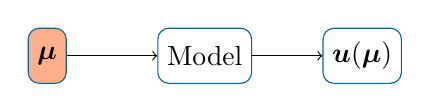
\begin{tikzpicture}[
      class/.style={rectangle, draw=darkblue, rounded corners, align=center, minimum height=0.7cm}
      ]
      \node[class, fill=salmon] (MU) at (-2,0) {$\bm \mu$};
      \node[class] (MOD) at (0,0) {Model};
      \node[class] (SOL) at (2,0) {$\bm u(\bm \mu)$};
      \draw[->] (MU.east) -- (MOD.west);
      \draw[->] (MOD.east) -- (SOL.west);
    \end{tikzpicture}
  \end{center}

  \begin{itemize}
  \item We are interested generating solutions $\bm u(\bm \mu)$ to a physical
    model that depend on a set of pre-determined \emph{parameters},
    $\bm\mu \in \mathcal{P}$.
  \item Parameters can be: viscosity, heat conductivity, varying boundary conditions, geometry
    changes, etc.
  \end{itemize}
\end{frame}

\begin{frame}
  \frametitle{Parameter-dependent models}

  Motivation: \emph{many-query} applications. E.g.~control systems, optimization, inverse problems and
  real-time responsiveness.

  \begin{center}
    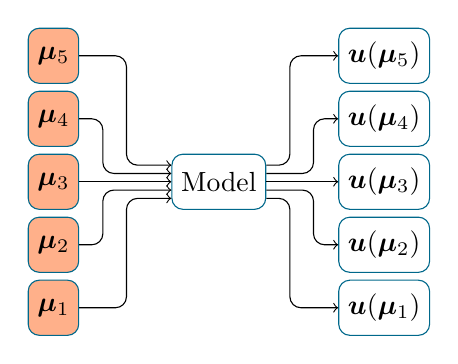
\begin{tikzpicture}[
      class/.style={rectangle, draw=darkblue, rounded corners, align=center, minimum height=0.7cm}
      ]
      \node[class, fill=salmon] (MU1) at (-2.1,-1.6) {$\bm \mu_1$};
      \node[class, fill=salmon] (MU2) at (-2.1,-0.8) {$\bm \mu_2$};
      \node[class, fill=salmon] (MU3) at (-2.1,0) {$\bm \mu_3$};
      \node[class, fill=salmon] (MU4) at (-2.1,0.8) {$\bm \mu_4$};
      \node[class, fill=salmon] (MU5) at (-2.1,1.6) {$\bm \mu_5$};
      \node[class] (MOD) at (0,0) {Model};
      \node[class] (SOL1) at (2.1,-1.6) {$\bm u(\bm \mu_1)$};
      \node[class] (SOL2) at (2.1,-0.8) {$\bm u(\bm \mu_2)$};
      \node[class] (SOL3) at (2.1,0) {$\bm u(\bm \mu_3)$};
      \node[class] (SOL4) at (2.1,0.8) {$\bm u(\bm \mu_4)$};
      \node[class] (SOL5) at (2.1,1.6) {$\bm u(\bm \mu_5)$};
      \draw[->,rounded corners] (MU1.east) -- ++(0.6,0) |- ([yshift=-6]MOD.west);
      \draw[->,rounded corners] (MU2.east) -- ++(0.3,0) |- ([yshift=-3]MOD.west);
      \draw[->] (MU3.east) -- (MOD.west);
      \draw[->,rounded corners] (MU4.east) -- ++(0.3,0) |- ([yshift=3]MOD.west);
      \draw[->,rounded corners] (MU5.east) -- ++(0.6,0) |- ([yshift=6]MOD.west);
      \draw[->,rounded corners] ([yshift=-6]MOD.east) -- ++(0.3,0) |- (SOL1.west);
      \draw[->,rounded corners] ([yshift=-3]MOD.east) -- ++(0.6,0) |- (SOL2.west);
      \draw[->] (MOD.east) -- (SOL3.west);
      \draw[->,rounded corners] ([yshift=3]MOD.east) -- ++(0.6,0) |- (SOL4.west);
      \draw[->,rounded corners] ([yshift=6]MOD.east) -- ++(0.3,0) |- (SOL5.west);
    \end{tikzpicture}
  \end{center}
\end{frame}

\begin{frame}
  \frametitle{Dimensional reduction}
  \begin{itemize}
  \item With conventional (read: FEM, FVM, FDM, and yes, even IGA) methods, this may be impractical
    if not impossible.
  \item Too many DoFs $N$ to finish in a realistic timeframe.
  \item Usually,
    \[ M = \dim \operatorname{``span''} \left( \left\{ \bm u(\bm \mu) \,|\, \bm \mu \in \mathcal{P} \right\} \right) \ll N \]
  \item Idea: create a model with number of DoFs closely matching the physical dimension of the
    problem.
  \item Often, $M \sim 100$ or so!
  \end{itemize}
\end{frame}

% \begin{frame}
%   \frametitle{Optimal reduced basis}

%   If we knew enough about ``typical'' solutions, we could create an optimal basis in the following
%   sense. \\~\\

%   Let $\mathcal{B} = \left\{ \bm b_1, \ldots, \bm b_M \right\}$ be a reduced basis, and let
%   $\mathcal{I}_{\mathcal{B}} : u(\mathcal{P}) \to \spann \mathcal{B}$ be the optimal-approximation
%   projection in some norm $\| \cdot \|_a$. Let
%   \[
%     \epsilon^2(\mathcal{B}) = \int_{\mathcal{P}}
%     \| \bm u(\mu) - \mathcal{I}_{\mathcal{B}} \bm u(\bm \mu) \|_a^2
%     \; \text{d} \bm \mu.
%   \]
%   Then $\mathcal{B_\text{opt}}$ is optimal if
%   \[
%     \epsilon(\mathcal{B}) < \epsilon(\mathcal{B_\text{opt}}) \Longrightarrow
%     \sharp \mathcal{B} > \sharp \mathcal{B}_\text{opt}.
%   \]
%   In other words, no other basis of the same size can achieve a better $\epsilon$.
% \end{frame}

% \begin{frame}
%   \frametitle{Good-enough reduced basis}

%   We can get close by employing \emph{Proper Orthogonal Decomposition} (POD) on a suitably large
%   \emph{ensemble} of \emph{snapshot} solutions. \\~\\

%   The reduced basis is then optimal in the discrete quadrature sense of
%   \[
%     \epsilon^2(\mathcal{B}) = \int_{\mathcal{P}}
%     \| \bm u(\mu) - \mathcal{I}_{\mathcal{B}} \bm u(\bm \mu) \|_a^2
%     \; \text{d} \bm \mu.
%   \]
%   In fact, the problem of choosing parameter values for our ensemble is equivalent to making a
%   quadrature rule on $\mathcal{P}$.
% \end{frame}

\begin{frame}
  \frametitle{The vision\footcite[See][]{Quarteroni2016rbm}}

  \begin{center}
    \begin{tikzpicture}[
      block/.style={
        minimum width=40mm,
        text width=38mm,
        align=center,
        rounded corners=1mm,
      },
      offline/.style={
        block,
        draw=darkblue,
        fill=cadet,
      },
      online/.style={
        block,
        draw=darkblue,
        fill=salmon,
      },
      clear/.style={
        block,
        draw=darkblue,
      },
      ]
      \node[offline] (pde) {\tiny Parametrized PDE};
      \node[offline, below=2mm of pde] (hifi) {
        \tiny
        High-fidelity discr. \\[0.5mm]
        $\bm A_h(\bm \mu) \bm u_h(\bm \mu) = \bm f_h(\bm \mu)$ \\[0.5mm]
        $\begin{aligned}
          \bm A_h(\bm \mu) &= \textstyle \sum_i \xi_i(\bm \mu) \bm A_i \\
          \bm f_h(\bm \mu) &= \textstyle \sum_i \chi_i(\bm \mu) \bm f_i
        \end{aligned}$
      };
      \node[offline, below=2mm of hifi] (snaps) {
        \tiny
        Generate a RB by applying POD to snapshot solutions, and construct
        projection matrix $\bm V$ \par
      };
      \node[offline, below=2mm of snaps] (proj) {
        \tiny
        Projection \\[1.0mm]
        $\begin{aligned}
          \bm A^M_i &= \bm V^\intercal \bm A_i \bm V \\
          \bm f^M_i &= \bm V^\intercal \bm f_i
        \end{aligned}$
      };
      \node[online, right=9mm of pde] (mu) {\tiny $\bm \mu$};
      \node[online, below=2mm of mu] (asm) {
        \tiny
        RB system assembly \\[1.0mm]
        $\begin{aligned}
          \bm A_M &= \textstyle \sum_i \xi_i(\bm \mu) \bm A^M_i \\
          \bm f_M &= \textstyle \sum_i \chi_i(\bm \mu) \bm f^M_i
        \end{aligned}$
      };
      \node[online, below=2mm of asm] (sol) {
        \tiny
        RB system solution \\[0.0mm]
        $\bm A_M(\bm \mu) \bm u_M(\bm \mu) = \bm f_M(\bm \mu)$
      };
      \node[clear, below=2mm of sol] (err) {
        \tiny
        Error estimate \\[0.0mm]
        $\| \bm u_h(\bm \mu) - \bm V \bm u_M(\bm \mu) \|$
      };
      \node[clear, below=2mm of err] (rec) {
        \tiny
        Recovery, visualization and post-processing \\[0.0mm]
        $\bm u_M^h(\bm \mu) = \bm V \bm u_M(\bm \mu)$
      };
      \node[clear, below=2mm of rec] (eval) {
        \tiny
        Evaluating functionals of interest
      };

      \draw[->] (pde.south) -- (hifi.north);
      \draw[->] (hifi.south) -- (snaps.north);
      \draw[->] (snaps.south) -- (proj.north);
      \draw[->] (mu.south) -- (asm.north);
      \draw[->, rounded corners] (proj.east) -- ($(proj.east) + (3mm,0)$) -- ($(asm.west) - (6mm,0)$) -- (asm.west);
      \draw[->] (asm.south) -- (sol.north);
      \draw[->, rounded corners] (sol.west) -- ($(sol.west) - (3mm,0)$) -- ($(eval.west) - (3mm,0)$) -- (eval.west);
      \draw[->] ($(err.west) - (3mm,0)$) -- (err.west);
      \draw[->] ($(rec.west) - (3mm,0)$) -- (rec.west);
    \end{tikzpicture}
  \end{center}
\end{frame}

\begin{frame}
  \begin{block}{\centering Our guiding principle}
    \begin{center}
      \vspace{5mm}
      ``\textbf{Any}'' extra cost in the offline stage is worth paying, \\
      no matter how much, if it makes the online stage faster. \\
      \vspace{5mm}
    \end{center}
  \end{block}
\end{frame}

\begin{frame}
  \begin{block}{\centering Our guiding principle}
    \begin{center}
      \vspace{5mm}
      All is fair in love, war \emph{and the offline stage}. \\
      --- John Lyly (\emph{Euphues}; 1579)
      \vspace{5mm}
    \end{center}
  \end{block}
\end{frame}

\begin{frame}
  \frametitle{Assembly}

  \begin{itemize}
  \item Why the insistence on forms like
    \[
      \bm A_h(\bm \mu) = \textstyle \sum_i \xi_i(\bm \mu) \bm A_i, \qquad
      \bm f_h(\bm \mu) = \textstyle \sum_i \chi_i(\bm \mu) \bm f_i
    \]
  \item Because it makes \emph{assembly} of reduced models fast.
  \item Each $\bm A_i$ and $\bm f_i$ can be projected independently onto a reduced basis and stored.
  \item This makes the online stage completely high-fidelity-agnostic.
  \item Deriving these \emph{affine representations} is the core detail of RBM.
  \end{itemize}
\end{frame}

\section{Stationary Navier-Stokes flow}

\begin{frame}
  \frametitle{Navier-Stokes equations}

  \begin{alignat*}{2}
    -\nu \Delta \bm u + (\bm u \cdot \nabla) \bm u + \nabla p &= \bm f && \qquad \text{in } \Omega, \\
    \nabla \cdot \bm u &= 0 && \qquad \text{in } \Omega, \\
    \bm u &= \bm g && \qquad \text{on } \Gamma_\text{D}, |\Gamma_D| > 0 \\
    -p \bm n + \nu (\nabla \bm u) \bm n &= \bm h && \qquad \text{on } \Gamma_\text{N}.
  \end{alignat*}
\end{frame}

\begin{frame}
  \frametitle{Divergence-conforming methods}

  \begin{itemize}
  \item Balance between velocity and pressure space is delicate.
  \item Too many velocity DoFs: poor enforcement of the continuity equation. Too many pressure DoFs:
    pressure instability.
  \item A pair of spaces $(V,P)$ is divergence-conforming if $\operatorname{div} V = P$. Ensures the strong
    (pointwise) form of the continuity equation, and no pressure instabilities.
  \item IGA unlocks easy construction of such spaces.\footcite{Buffa2010iae,Evans2013idc1}
  \end{itemize}
\end{frame}

\begin{frame}
  \frametitle{Anatomy of a reduced system}

  \begin{center}
    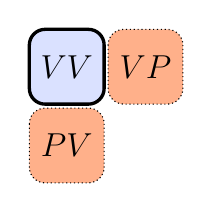
\begin{tikzpicture}[scale=1]
      \fill[cadet, draw=black, very thick, rounded corners=2mm] (0,-0.5) rectangle (0.95,-1.45);
      \fill[salmon, draw=black, densely dotted, rounded corners=2mm] (1,-0.5) rectangle (1.95,-1.45);
      \fill[salmon, draw=black, densely dotted, rounded corners=2mm] (0,-1.5) rectangle (0.95,-2.45);
      \node at (0.475,-0.975) {\large $VV$};
      \node at (1.475,-0.975) {\large $VP$};
      \node at (0.475,-1.975) {\large $PV$};
    \end{tikzpicture}
  \end{center}

  \begin{itemize}
  \item Usually, the reduced method does not inherit the stability properties of the high-fidelity
    method.
  \item Rank-deficient velocity-pressure blocks are common.
  \item Carefully selecting number of velocity modes and pressure modes seems to help?
    \[
      M_\textsc{v} \approx d M_\textsc{p}
    \]
  \end{itemize}
\end{frame}

\begin{frame}
  \frametitle{Anatomy of a reduced system (cont.)}

  \begin{center}
    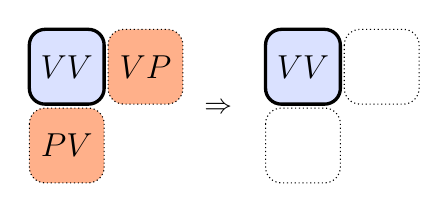
\begin{tikzpicture}[scale=1]
      \fill[cadet, draw=black, very thick, rounded corners=2mm] (0,-0.5) rectangle (0.95,-1.45);
      \fill[salmon, draw=black, densely dotted, rounded corners=2mm] (1,-0.5) rectangle (1.95,-1.45);
      \fill[salmon, draw=black, densely dotted, rounded corners=2mm] (0,-1.5) rectangle (0.95,-2.45);
      \node at (0.475,-0.975) {\large $VV$};
      \node at (1.475,-0.975) {\large $VP$};
      \node at (0.475,-1.975) {\large $PV$};

      \node at (2.4,-1.5) {$\Rightarrow$};

      \fill[cadet, draw=black, very thick, rounded corners=2mm] (3,-0.5) rectangle (3.95,-1.45);
      \draw[black, densely dotted, rounded corners=2mm] (4,-0.5) rectangle (4.95,-1.45);
      \draw[black, densely dotted, rounded corners=2mm] (3,-1.5) rectangle (3.95,-2.45);
      \node at (3.475,-0.975) {\large $VV$};
    \end{tikzpicture}
  \end{center}

  \begin{itemize}
  \item A divergence-free reduced basis eliminates the coupling, leading to a fully stable
    velocity-only formulation.
  \item IGA\footcite{Hughes2005iac,Cottrell2009iat} enables divergence-free high-fidelity
    solutions,\footcite{Evans2013idc1} therefore also divergence-free reduced bases.
  \end{itemize}
\end{frame}

\begin{frame}
  \frametitle{Divergence-free basis}

  \begin{center}
    \begin{tikzpicture}[
      block/.style={
        minimum width=40mm,
        minimum height=8mm,
        align=center,
        rounded corners,
        fill=cadet,
        draw=darkblue,
      }
      ]
      \node[block] (HIFI) at (0,6.4) {Hi-Fi solutions};
      \node[block] (RGEOM) at (0,5.2) {Reference geometry};
      \node[block] (UNLIF) at (0,4) {Unlifted solutions};
      \node[block,fill=salmon] (POD) at (0,2.8) {POD};
      \node[block] (RB) at (0,1.6) {Reduced basis};

      \draw[->] (HIFI.south) -- (RGEOM.north);
      \draw[->] (RGEOM.south) -- (UNLIF.north);
      \draw[->] (UNLIF.south) -- (POD.north);
      \draw[->] (POD.south) -- (RB.north);

      \only<1-6>{\node[anchor=west,white] at (3.5,6.4) {Divergence-conforming};}
      \only<2>{\node[anchor=west] at (3.5,6.4) {Divergence-conforming};}
      \only<3-6>{\node[anchor=west,gray] at (3.5,6.4) {Divergence-conforming};}
      \only<3>{\node[anchor=west] at (3.5,5.2) {Piola transform};}
      \only<4-6>{\node[anchor=west,gray] at (3.5,5.2) {Piola transform};}
      \only<4>{\node[anchor=west] at (3.5,4.0) {Divergence-free lift};}
      \only<5-6>{\node[anchor=west,gray] at (3.5,4.0) {Divergence-free lift};}
      \only<5>{\node[anchor=west] at (3.5,2.8) {Linearity};}
      \only<6>{\node[anchor=west,gray] at (3.5,2.8) {Linearity};}
      \only<6>{\node[anchor=west] at (3.5,1.6) {Divergence-free basis};}
      \only<2>{\draw[->, very thick, darkblue] (3.5,6.4) -- (HIFI.east);}
      \only<3>{\draw[->, very thick, darkblue] (3.5,5.2) -- (RGEOM.east);}
      \only<4>{\draw[->, very thick, darkblue] (3.5,4) -- (UNLIF.east);}
      \only<5>{\draw[->, very thick, darkblue] (3.5,2.8) -- (POD.east);}
      \only<6>{\draw[->, very thick, darkblue] (3.5,1.6) -- (RB.east);}
    \end{tikzpicture}
  \end{center}
\end{frame}

\section{Pressure recovery}

\begin{frame}
  \frametitle{Pressure recovery}

  \begin{itemize}
  \item The simplest approach is to attach pressure data to divergence-free velocity basis
    functions.
  \item Pressure recovery becomes ``free'' (no linear system to solve, use coefficients from RB
    velocity solution).
  \item However, this implies a linear velocity-pressure relationship, in violation of
    e.g.~Navier-Stokes.
  \item Could work depending on problem.
  \end{itemize}
\end{frame}

\begin{frame}
  \frametitle{Pressure recovery}

  \begin{itemize}
  \item Another approach is to solve the momentum equation with a different test space.
  \item The ``optimal'' test functions are \emph{supremizers}, maximizers of the ``sup'' part of the
    inf-sup condition, for any specific pressure solution.
  \item Supremizers form a reduced space just like velocity and pressure do.
  \item Supremizers are commonly used to enrich non-divergence-free reduced velocity spaces for stability.
    \footcite{Ballarin2015ssp}
  \end{itemize}
\end{frame}

\begin{frame}
  \frametitle{Anatomy of a reduced system (cont.)}

  \begin{center}
    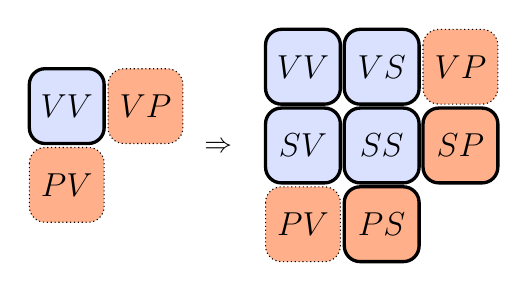
\begin{tikzpicture}[scale=1]
      \fill[cadet, draw=black, very thick, rounded corners=2mm] (0,-0.5) rectangle (0.95,-1.45);
      \fill[salmon, draw=black, densely dotted, rounded corners=2mm] (1,-0.5) rectangle (1.95,-1.45);
      \fill[salmon, draw=black, densely dotted, rounded corners=2mm] (0,-1.5) rectangle (0.95,-2.45);
      \node at (0.475,-0.975) {\large $VV$};
      \node at (1.475,-0.975) {\large $VP$};
      \node at (0.475,-1.975) {\large $PV$};

      \node at (2.4,-1.5) {$\Rightarrow$};

      \fill[cadet, draw=black, very thick, rounded corners=2mm] (3,0) rectangle (3.95,-0.95);
      \fill[cadet, draw=black, very thick, rounded corners=2mm] (4,0) rectangle (4.95,-0.95);
      \fill[cadet, draw=black, very thick, rounded corners=2mm] (3,-1) rectangle (3.95,-1.95);
      \fill[cadet, draw=black, very thick, rounded corners=2mm] (4,-1) rectangle (4.95,-1.95);
      \fill[salmon, draw=black, densely dotted, rounded corners=2mm] (5,0) rectangle (5.95,-0.95);
      \fill[salmon, draw=black, densely dotted, rounded corners=2mm] (3,-2) rectangle (3.95,-2.95);
      \fill[salmon, draw=black, very thick, rounded corners=2mm] (5,-1) rectangle (5.95,-1.95);
      \fill[salmon, draw=black, very thick, rounded corners=2mm] (4,-2) rectangle (4.95,-2.95);
      \node at (3.475,-0.475) {\large $VV$};
      \node at (4.475,-0.475) {\large $VS$};
      \node at (5.475,-0.475) {\large $VP$};
      \node at (3.475,-1.475) {\large $SV$};
      \node at (4.475,-1.475) {\large $SS$};
      \node at (5.475,-1.475) {\large $SP$};
      \node at (3.475,-2.475) {\large $PV$};
      \node at (4.475,-2.475) {\large $PS$};
    \end{tikzpicture}
    \\~\\
    \textcolor{white}{Note the block triangular structure.}
  \end{center}
\end{frame}

\begin{frame}
  \frametitle{Anatomy of a reduced system (cont.)}

  \begin{center}
    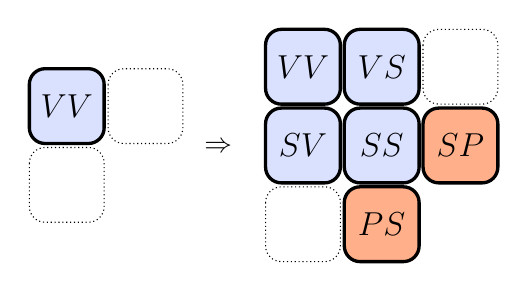
\begin{tikzpicture}[scale=1]
      \fill[cadet, draw=black, very thick, rounded corners=2mm] (7,-0.5) rectangle (7.95,-1.45);
      \draw[black, densely dotted, rounded corners=2mm] (8,-0.5) rectangle (8.95,-1.45);
      \draw[black, densely dotted, rounded corners=2mm] (7,-1.5) rectangle (7.95,-2.45);
      \node at (7.475,-0.975) {\large $VV$};

      \node at (9.4,-1.5) {$\Rightarrow$};

      \fill[cadet, draw=black, very thick, rounded corners=2mm] (10,0) rectangle (10.95,-0.95);
      \fill[cadet, draw=black, very thick, rounded corners=2mm] (11,0) rectangle (11.95,-0.95);
      \fill[cadet, draw=black, very thick, rounded corners=2mm] (10,-1) rectangle (10.95,-1.95);
      \fill[cadet, draw=black, very thick, rounded corners=2mm] (11,-1) rectangle (11.95,-1.95);
      \draw[black, densely dotted, rounded corners=2mm] (12,0) rectangle (12.95,-0.95);
      \draw[black, densely dotted, rounded corners=2mm] (10,-2) rectangle (10.95,-2.95);
      \fill[salmon, draw=black, very thick, rounded corners=2mm] (12,-1) rectangle (12.95,-1.95);
      \fill[salmon, draw=black, very thick, rounded corners=2mm] (11,-2) rectangle (11.95,-2.95);
      \node at (10.475,-0.475) {\large $VV$};
      \node at (11.475,-0.475) {\large $VS$};
      \node at (10.475,-1.475) {\large $SV$};
      \node at (11.475,-1.475) {\large $SS$};
      \node at (12.475,-1.475) {\large $SP$};
      \node at (11.475,-2.475) {\large $PS$};
    \end{tikzpicture}
    \\~\\
    Note the block triangular structure.
  \end{center}
\end{frame}

\section{Numerical examples}

\begin{frame}
  \frametitle{Flow around airfoil}

  \begin{center}
    \begin{tikzpicture}
      \draw[densely dotted, thick] (0,-3) arc (-90:90:3);
      \draw[thick] (0,3) arc (90:270:3);
      \draw[->] (-3,0) -- (-2.2,0);
      \draw[->] (-2.93,0.6) -- (-2.13,0.6);
      \draw[->] (-2.75,1.2) -- (-1.95,1.2);
      \draw[->] (-2.40,1.8) -- (-1.60,1.8);
      \draw[->] (-1.80,2.4) -- (-1.00,2.4);
      \draw[->] (-2.93,-0.6) -- (-2.13,-0.6);
      \draw[->] (-2.75,-1.2) -- (-1.95,-1.2);
      \draw[->] (-2.40,-1.8) -- (-1.60,-1.8);
      \draw[->] (-1.80,-2.4) -- (-1.00,-2.4);
      \node[anchor=east] at (-3,0) {$\bm u_\infty$};
      \draw[->] (1.6,0) arc (0:30:1.6);
      \draw[->] (1.6,0) arc (0:-30:1.6);
      \node[anchor=west] at (1.6,0) {$\varphi$};
      \begin{scope}[scale=0.3, shift={(-3,-1.4)}]
        \begin{axis}[xmin=-0.01, xmax=1.01, ymin=-0.2, ymax=0.2, unit vector ratio*=1 1, axis lines=none]
          \addplot[black, line width=2.5]
          table[x index={0}, y index={1}]{data/NACApts.dat};
        \end{axis}
      \end{scope}
      \begin{scope}[scale=0.3, rotate=30, shift={(-3,-1.5)}]
        \begin{axis}[xmin=-0.01, xmax=1.01, ymin=-0.2, ymax=0.2, unit vector ratio*=1 1, axis lines=none]
          \addplot[black, line width=1.5, dotted]
          table[x index={0}, y index={1}]{data/NACApts.dat};
        \end{axis}
      \end{scope}
      \begin{scope}[scale=0.3, rotate=-30, shift={(-3,-1.3)}]
        \begin{axis}[xmin=-0.01, xmax=1.01, ymin=-0.2, ymax=0.2, unit vector ratio*=1 1, axis lines=none]
          \addplot[black, line width=1.5, dotted]
          table[x index={0}, y index={1}]{data/NACApts.dat};
        \end{axis}
      \end{scope}
    \end{tikzpicture}
  \end{center}
\end{frame}

\begin{frame}
  \frametitle{Domain transformation}

  \begin{center}
    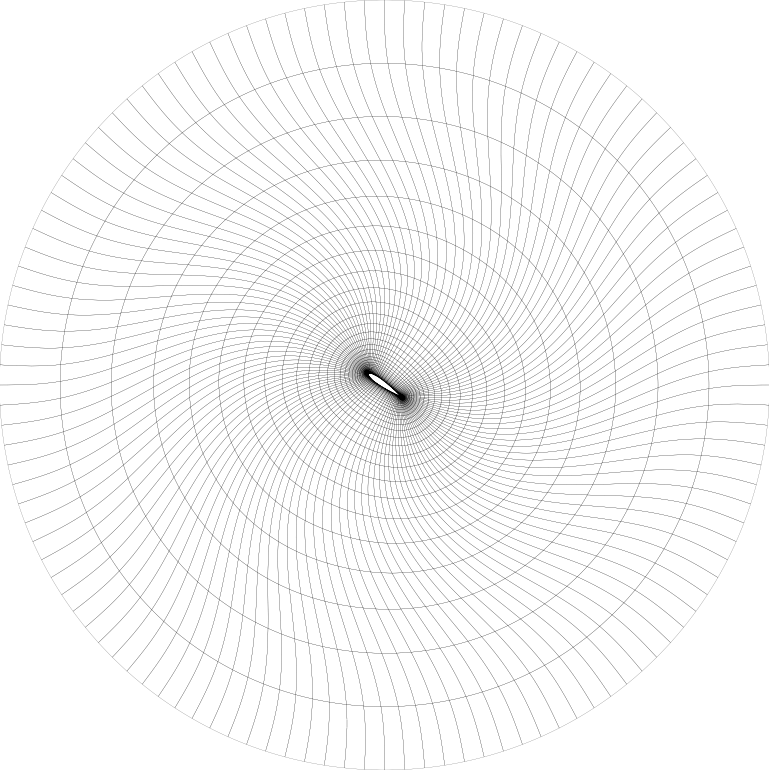
\includegraphics[width=0.8\textheight]{figs/domain}
  \end{center}
\end{frame}

\begin{frame}
  \frametitle{Parameter space}

  \begin{center}
    \begin{tikzpicture}[scale=6]
      \draw[very thick, ->] (0,0) -- (1,0);
      \draw[very thick, ->] (0,0) -- (0,1);
      \node[anchor=south west] at (0,0) {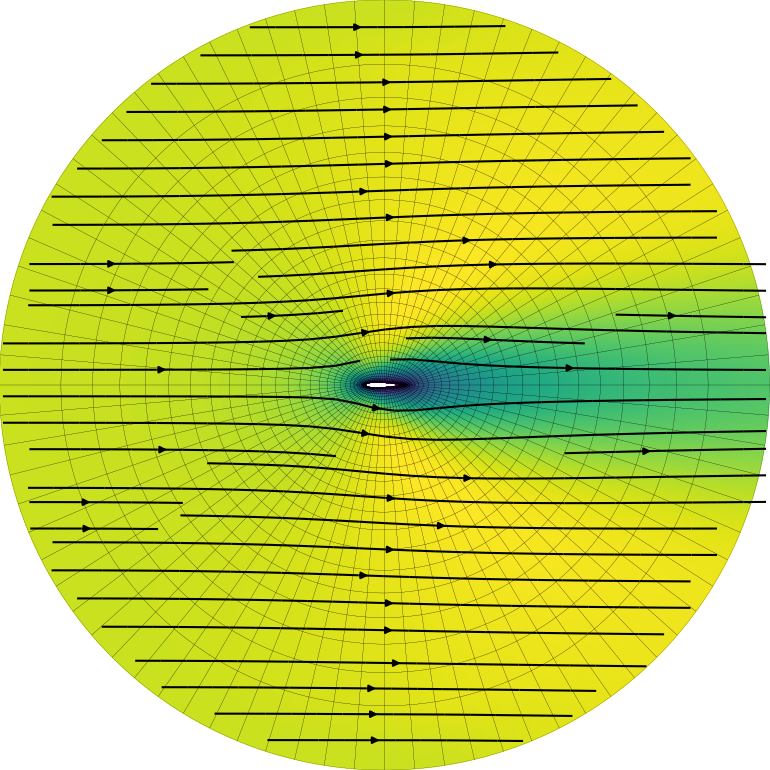
\includegraphics[width=28mm]{figs/full-lo-lo}};
      \node[anchor=south east] at (1,0) {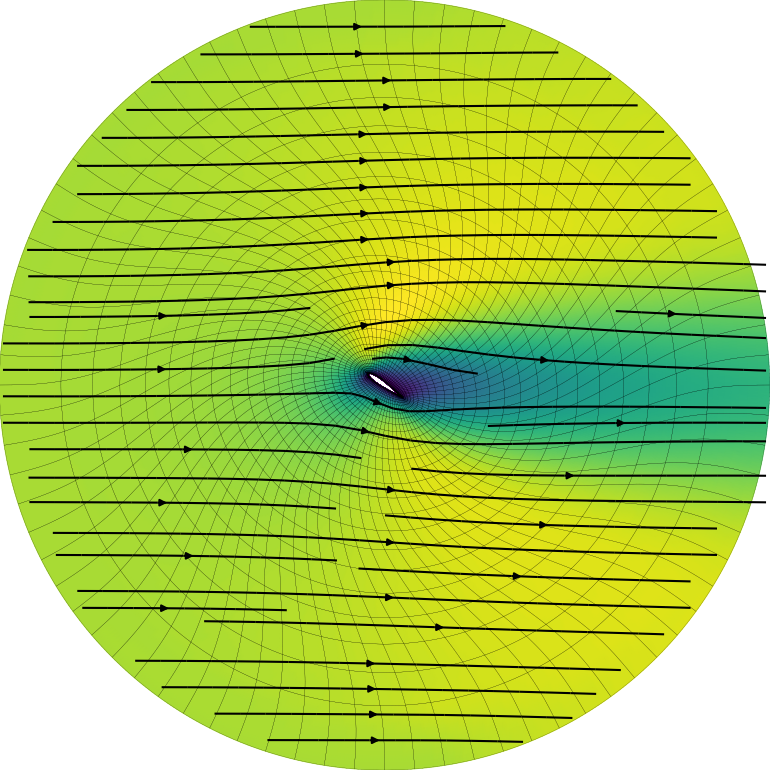
\includegraphics[width=28mm]{figs/full-hi-lo}};
      \node[anchor=north east] at (1,1) {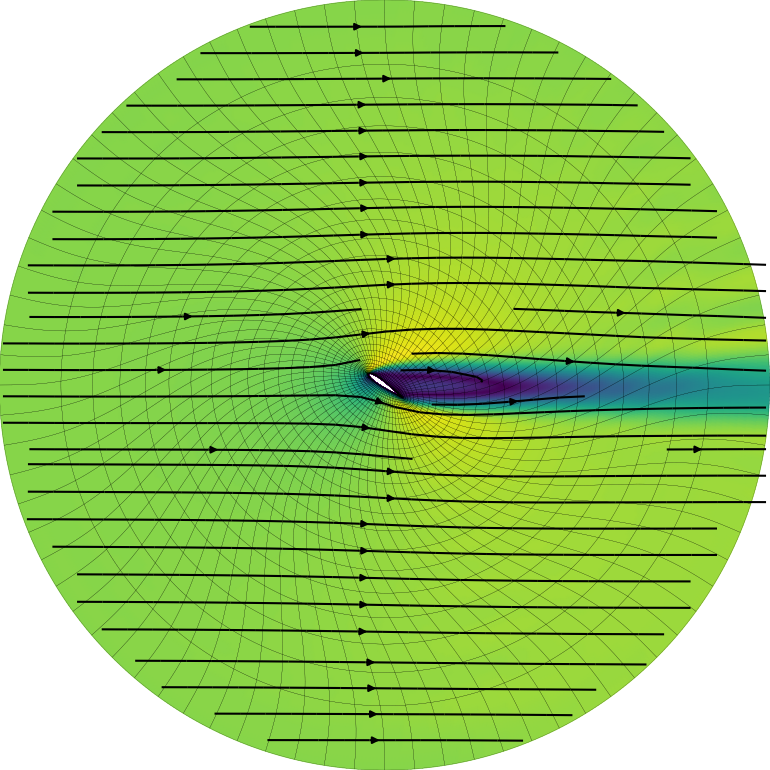
\includegraphics[width=28mm]{figs/full-hi-hi}};
      \node[anchor=north west] at (0,1) {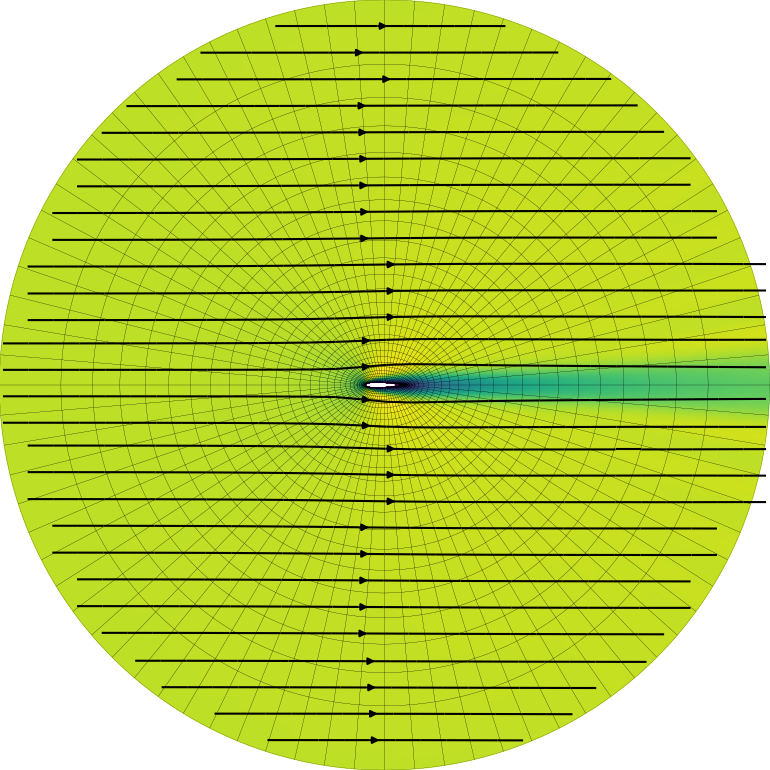
\includegraphics[width=28mm]{figs/full-lo-hi}};
      \node[anchor=north] at (0.5,0) {Angle of attack ($\varphi$)};
      \node[anchor=south, rotate=90] at (0,0.5) {Airspeed ($u_\infty$)};
    \end{tikzpicture}
  \end{center}
\end{frame}

\begin{frame}
  \frametitle{Problem specification}

  \begin{itemize}
  \item We will try two high-fidelity methods: a Taylor-Hood (1,2)-method and an IGA (1,2)
    divergence-conforming method, with both approaches to pressure recovery.
  \item The parameter domain was chosen as
    \[
      \mathcal{P} = [-\SI{35}{\degree}, +\SI{35}{\degree}] \times
      [\SI{1}{\meter/\second}, \SI{20}{\meter/\second}].
    \]
  \item Only \emph{stationary} Navier-Stokes, with $\nu = \frac{1}{6}$.
  \item We chose equal number of modes in all spaces: $N_\textsc{v} = N_\textsc{s} = N_\textsc{p} = M$.
  \end{itemize}
\end{frame}

\begin{frame}
  \frametitle{Affine representations}

  \begin{itemize}
  \item Not possible to express the Navier-Stokes problem as finite sums
    \[
      \bm A_h(\bm \mu) = \textstyle \sum_i \xi_i(\bm \mu) \bm A_i, \qquad
      \bm f_h(\bm \mu) = \textstyle \sum_i \chi_i(\bm \mu) \bm f_i
    \]
  \item Instead, we use truncated polynomial series in $\varphi$.\footcite{Fonn2018fdc}
  \item We can expect about $10$ digits of accuracy with a reasonable number of terms
    (${\sim}25$ for TH, ${\sim}75$ for DC).
  \item Recall: the intention is to encode \emph{all} parameters explicitly in the representation of
    the bi- or trilinear forms.
  \end{itemize}

  \[
    \bm J = \sum_i \varphi^i \bm B_i^{(+)}
    \qquad \bm J^{-\intercal} = \sum_i \varphi_j \bm B_j^{(-)}
  \]
  \[
    \bm J^{-1} \bm J^{-\intercal} = \bm I + \varphi \bm D_1 - \varphi^2 \bm D_2
  \]
\end{frame}

\begin{frame}
  \frametitle{Affine representations (TH)}
  \begin{align*}
    ({\bm\pi}^*_{\bm\mu}a)(\hat{\bm u}, \hat{\bm w}; \varphi) &=
    \nu \int_{\hat{\Omega}} \nabla \hat{\bm u} : \nabla \hat{\bm w}
    + \nu \varphi \int_{\hat{\Omega}}
    \nabla \hat{\bm u} : (\bm D_1 \nabla) \hat{\bm w} \\
    &- \nu \varphi^2 \int_{\hat{\Omega}}
    \nabla \hat{\bm u} : (\bm D_2 \nabla) \hat{\bm w} \\
    ({\bm\pi}^*_{\bm\mu}b)(\hat{p}, \hat{\bm w}; \varphi) &\approx \sum_{i=0}^{2n} \varphi^i
    \int_{\hat{\Omega}} \hat{p} \bm B^{(-)}_i : \nabla \hat{\bm w} \\
    ({\bm\pi}^*_{\bm\mu}c)(\hat{\bm u}, \hat{\bm v}, \hat{\bm w}; \varphi)
    &\approx \sum_{i=0}^{2n} \varphi^i \int_{\hat{\Omega}}
    (\hat{\bm u} \cdot \bm B^{(-)}_i \nabla) \hat{\bm v} \cdot \hat{\bm w}
  \end{align*}
\end{frame}

\begin{frame}
  \frametitle{Affine representations (IGA)}

  \begin{align*}
  ({\bm\pi}^*_{\bm\mu}a)(\hat{\bm u}, \hat{\bm w}; \varphi)
    &= \nu \sum_{i,j=0}^{2n} \varphi^{i+j} \int_{\hat{\Omega}}
      \nabla (\bm B^{(+)}_i \hat{\bm u}) : \nabla (\bm B^{(+)}_j \hat{\bm w}) \\
    &+ \nu \sum_{i,j=0}^{2n} \varphi^{i+j+1} \int_{\hat{\Omega}}
      \nabla (\bm B^{(+)}_i \hat{\bm u}) : (\bm D_1 \nabla) (\bm B^{(+)}_j \hat{\bm w}) \\
    &- \sum_{i,j=0}^{2n} \varphi^{i+j+2} \int_{\hat{\Omega}}
      \nabla (\bm B^{(+)}_i \hat{\bm u}) : (\bm D_2 \nabla) (\bm B^{(+)}_j \hat{\bm w}) \\
  ({\bm\pi}^*_{\bm\mu}b)(\hat{p}, \hat{\bm w}; \varphi) &= \sum_{i,j=0}^{2n} \varphi^{i+j}
      \int_{\hat{\Omega}} \hat{p} \bm B^{(-)}_i :
      \nabla \left( \bm B^{(+)}_j \hat{\bm w} \right) \\
  ({\bm\pi}^*_{\bm\mu}c)(\hat{\bm u}, \hat{\bm v}, \hat{\bm w}; \varphi)
  &= \sum_{i,j=0}^{2n} \varphi^{i+j}
    \int_{\hat{\Omega}} (\hat{\bm u} \cdot \nabla) \bm B^{(+)}_i \hat{\bm v} \cdot \bm B^{(+)}_j \hat{\bm w}.
  \end{align*}
\end{frame}

\section{Results}

\begin{frame}
  \frametitle{Spectrum}

  \begin{center}
    \begin{tikzpicture}
      \begin{axis}[
        xlabel={$k$},
        ylabel={$\lambda_k$},
        ymode=log,
        xmin=0, xmax=225,
        width=0.9\textwidth,
        height=0.6\textwidth,
        grid=both,
        axis lines=left,
        legend style={
          at={(1, 1)},
          anchor=north east,
          font=\small,
        },
        legend cell align=left,
        ]
        \addplot[red, thick]
        table[x index={0}, y index={1}]{data/airfoil-spectrum-no-piola.csv};
        \addplot[blue, thick]
        table[x index={0}, y index={2}]{data/airfoil-spectrum-no-piola.csv};
        \addplot[green, thick]
        table[x index={0}, y index={3}]{data/airfoil-spectrum-no-piola.csv};
        \addplot[red, thick, dashed]
        table[x index={0}, y index={1}]{data/airfoil-spectrum-piola.csv};
        \addplot[blue, thick, dashed]
        table[x index={0}, y index={2}]{data/airfoil-spectrum-piola.csv};
        \addplot[green, thick, dashed]
        table[x index={0}, y index={3}]{data/airfoil-spectrum-piola.csv};
        \legend{TH ($v$), TH ($p$), TH (sup), DC ($v$), DC ($p$), DC (sup)}
      \end{axis}
    \end{tikzpicture}
  \end{center}
\end{frame}

\begin{frame}
  \frametitle{Basis functions (v, TH, \only<1>{1}\only<2>{2}\only<3>{3}\only<4>{4})}

  \begin{center}
    \only<1>{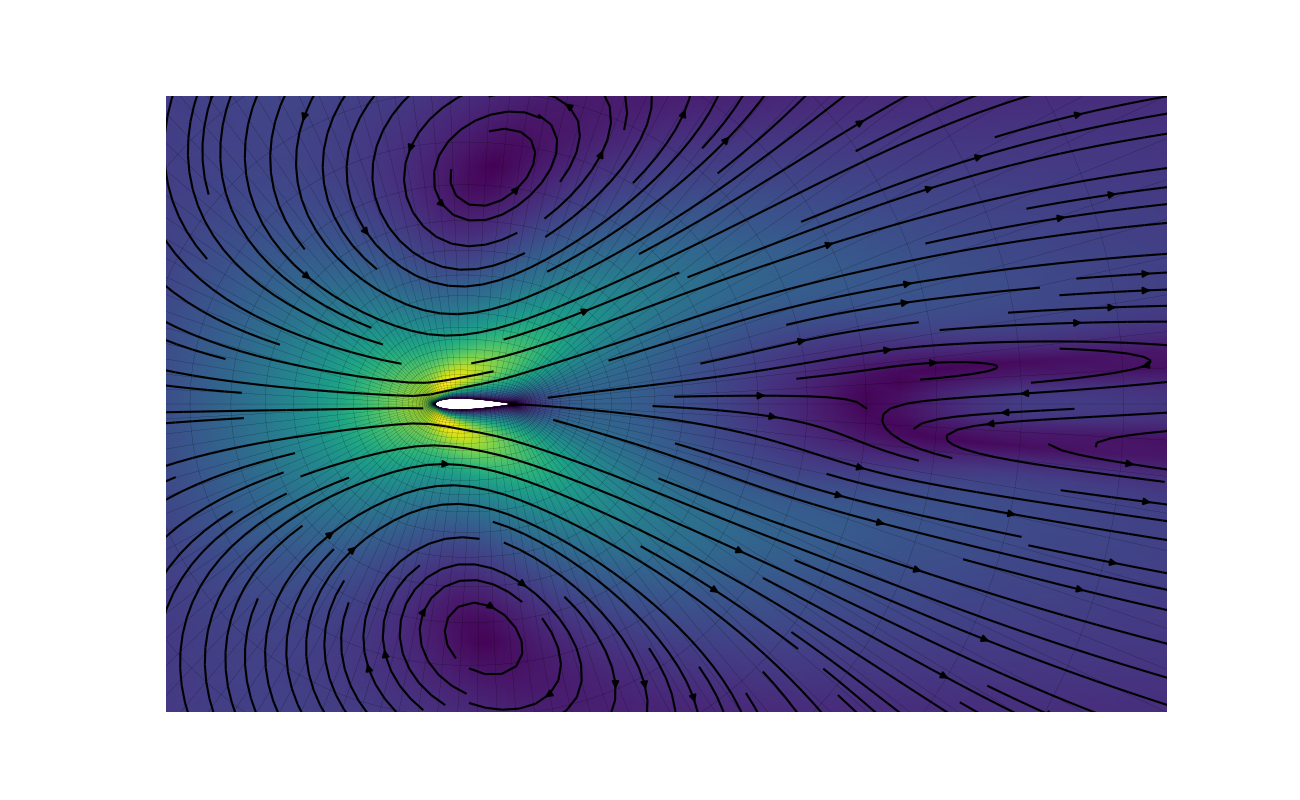
\includegraphics[width=1.0\textwidth]{figs/bfun-v-no-piola-v000}
    }\only<2>{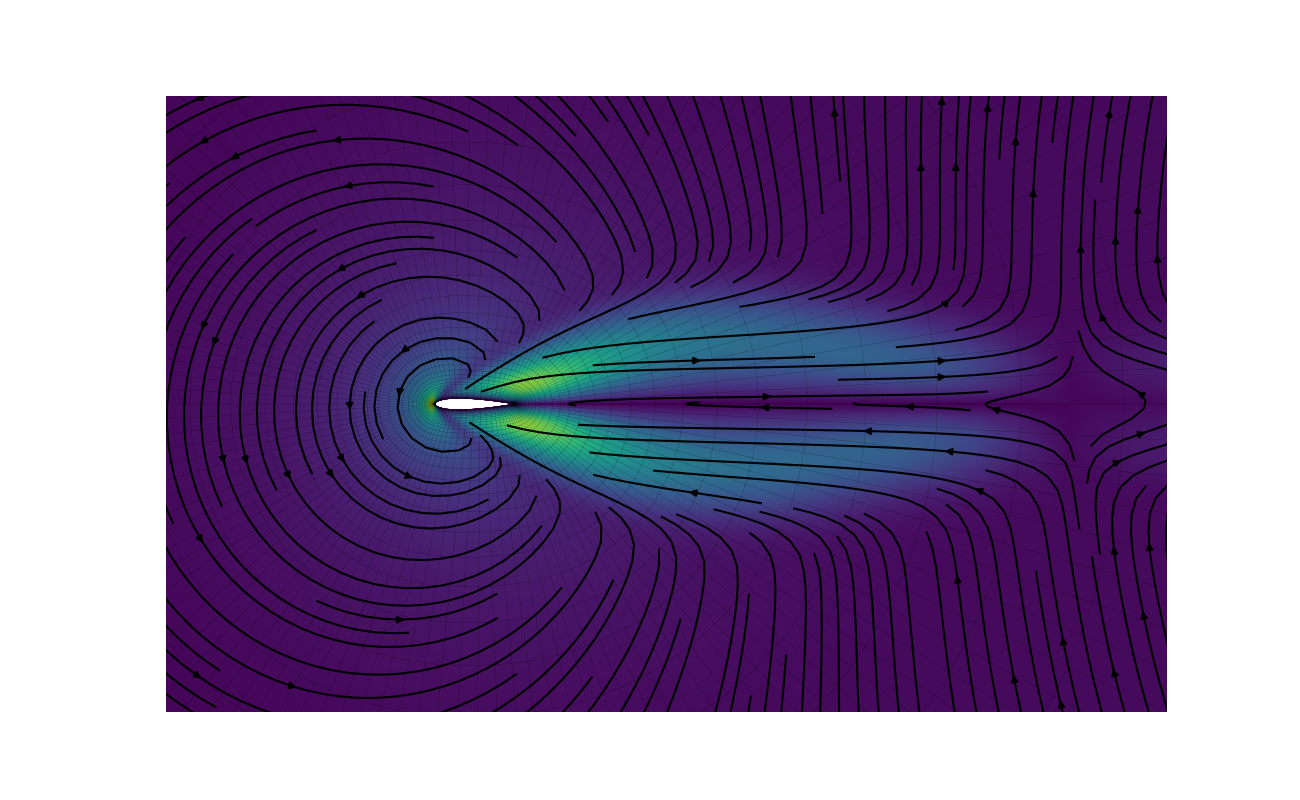
\includegraphics[width=1.0\textwidth]{figs/bfun-v-no-piola-v001}
    }\only<3>{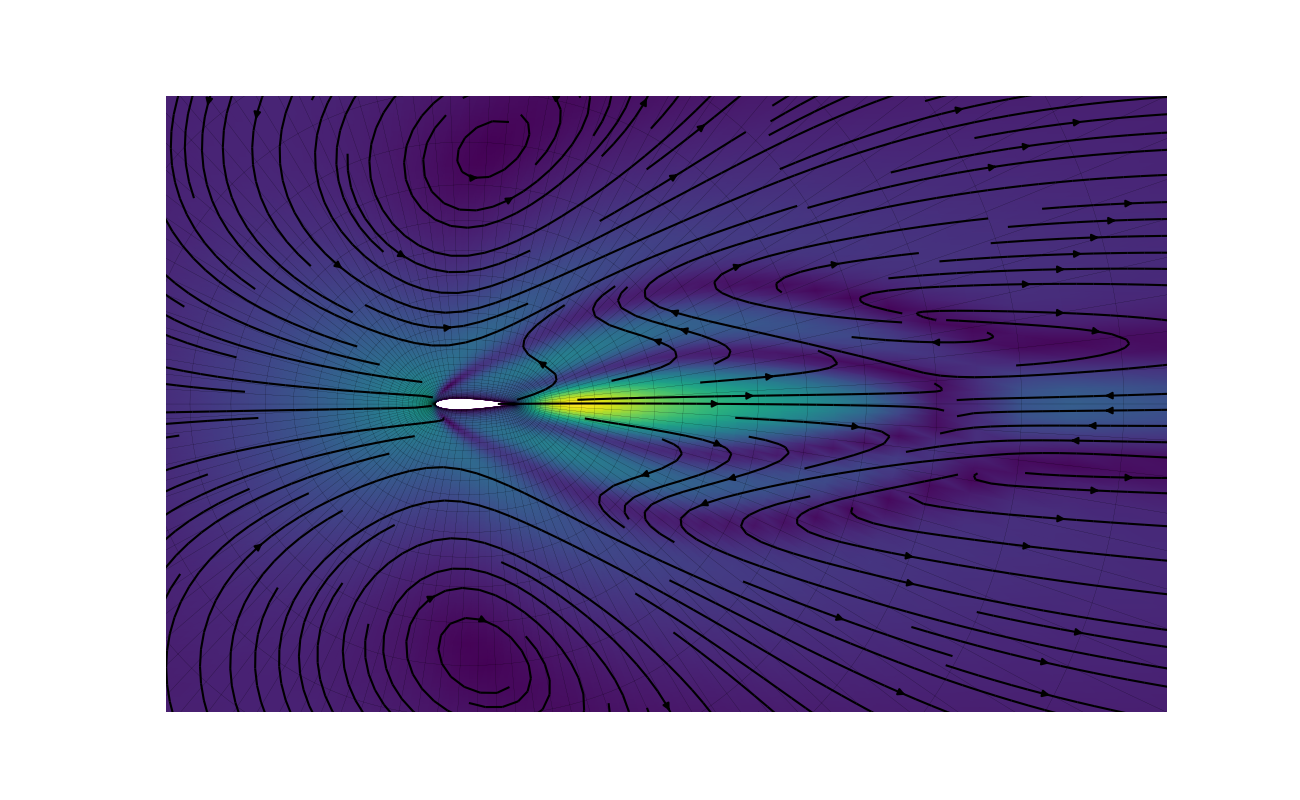
\includegraphics[width=1.0\textwidth]{figs/bfun-v-no-piola-v002}
    }\only<4>{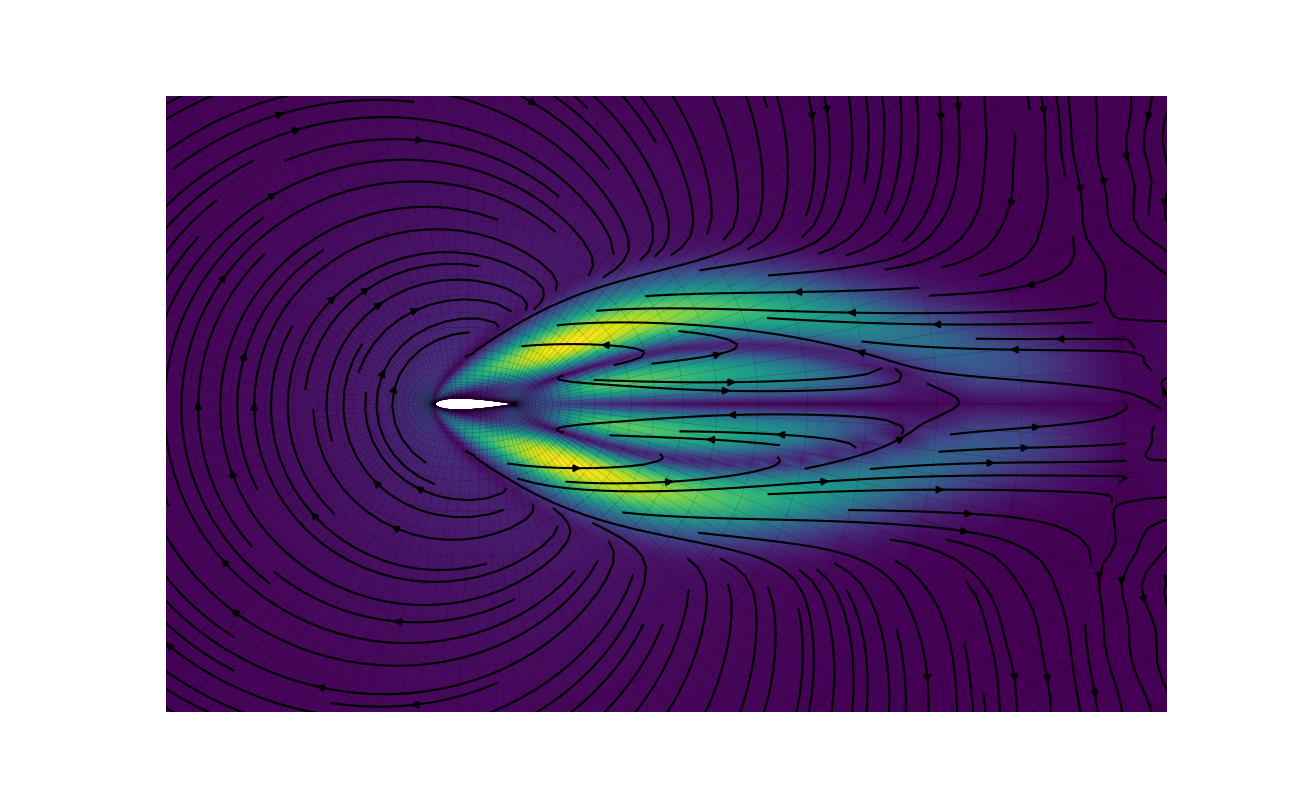
\includegraphics[width=1.0\textwidth]{figs/bfun-v-no-piola-v003}}
  \end{center}
\end{frame}

\begin{frame}
  \frametitle{Basis functions (v, DC, \only<1>{1}\only<2>{2}\only<3>{3}\only<4>{4})}

  \begin{center}
    \only<1>{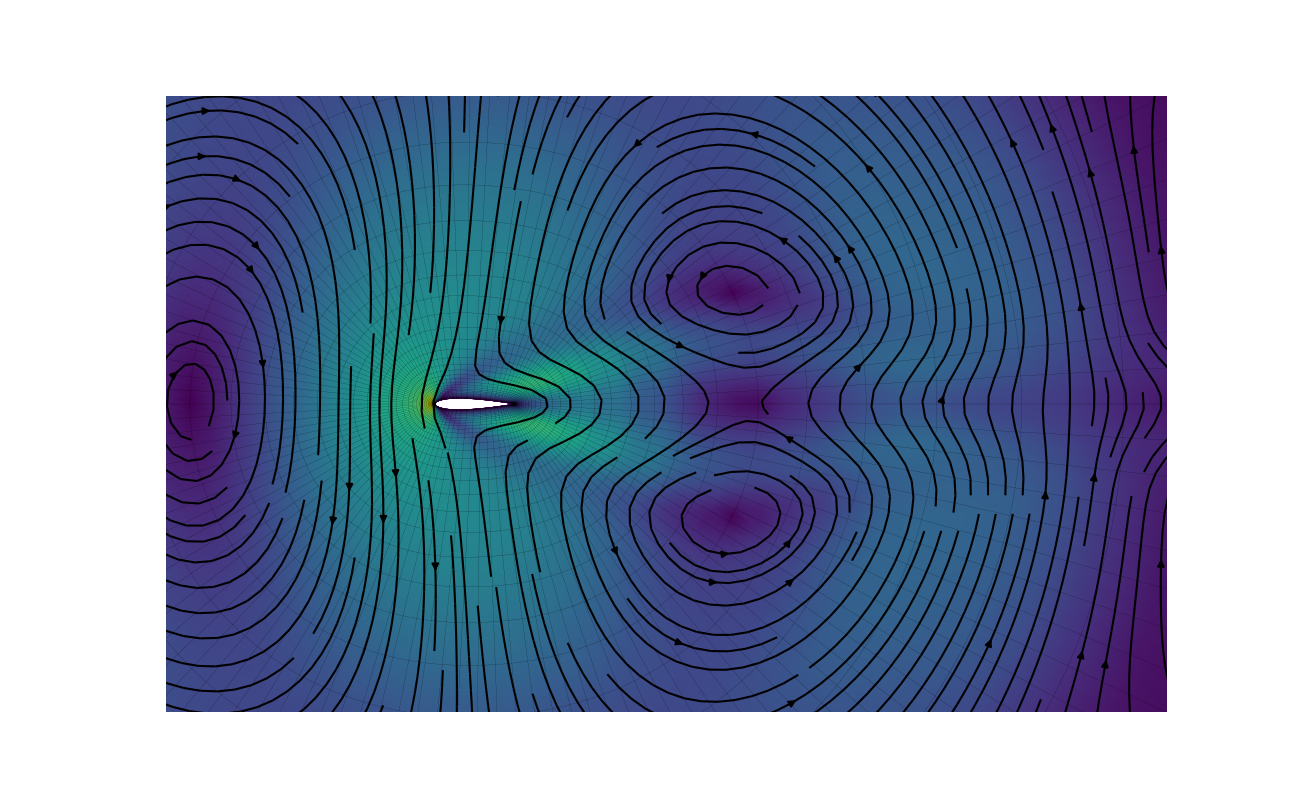
\includegraphics[width=1.0\textwidth]{figs/bfun-v-piola-v000}
    }\only<2>{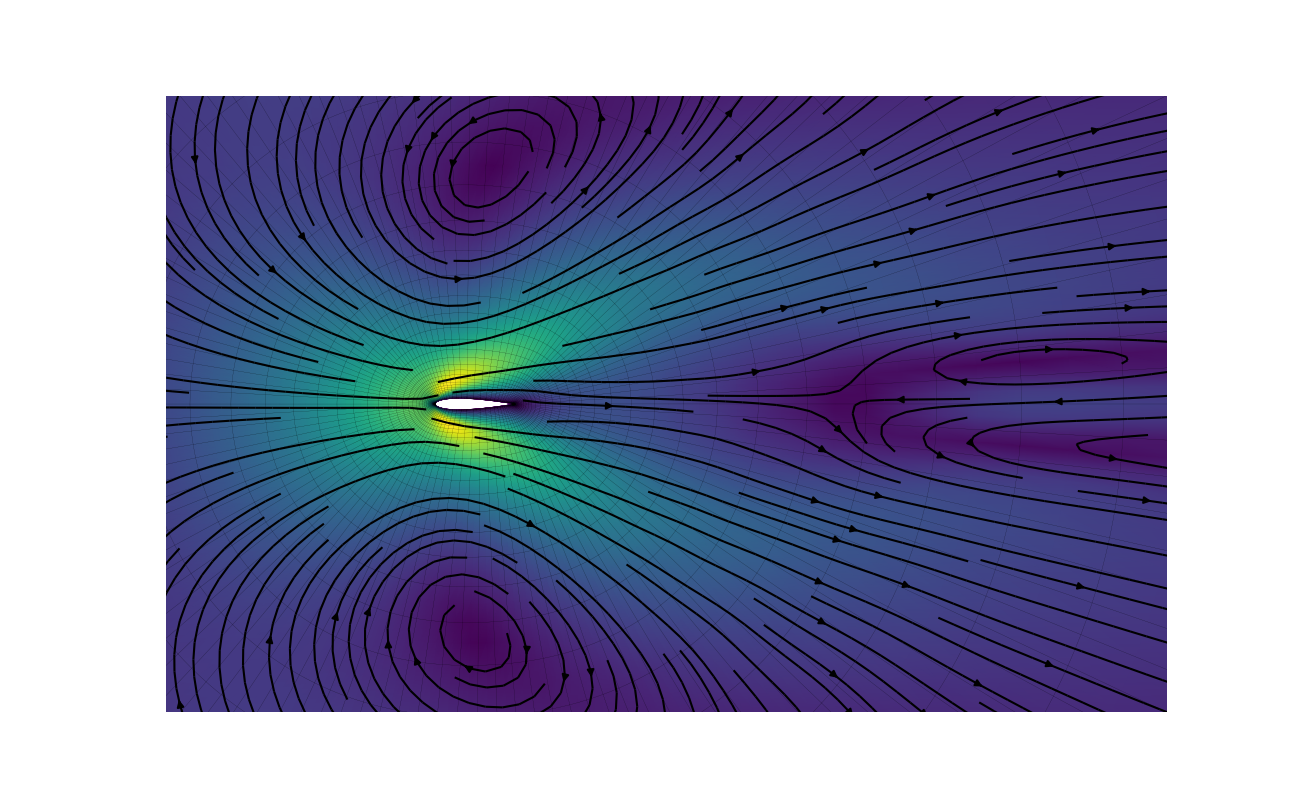
\includegraphics[width=1.0\textwidth]{figs/bfun-v-piola-v001}
    }\only<3>{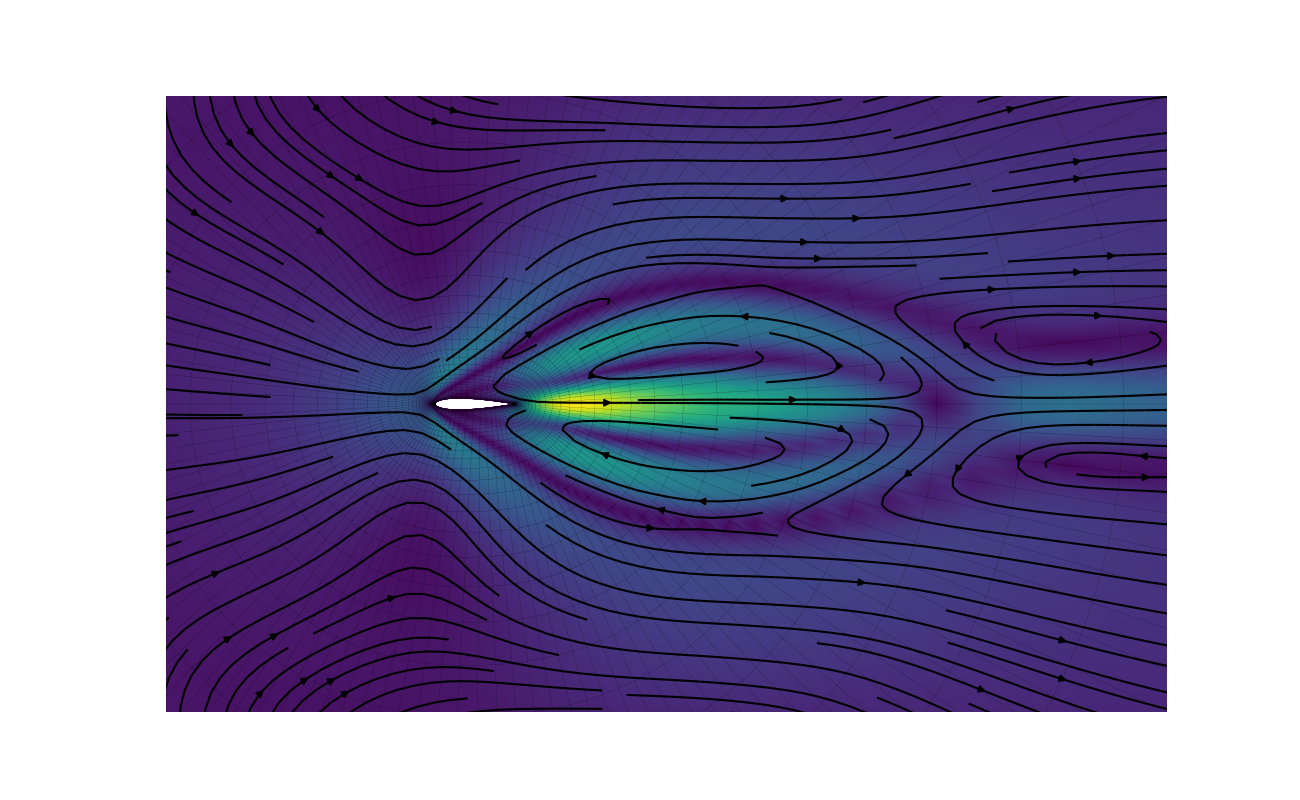
\includegraphics[width=1.0\textwidth]{figs/bfun-v-piola-v002}
    }\only<4>{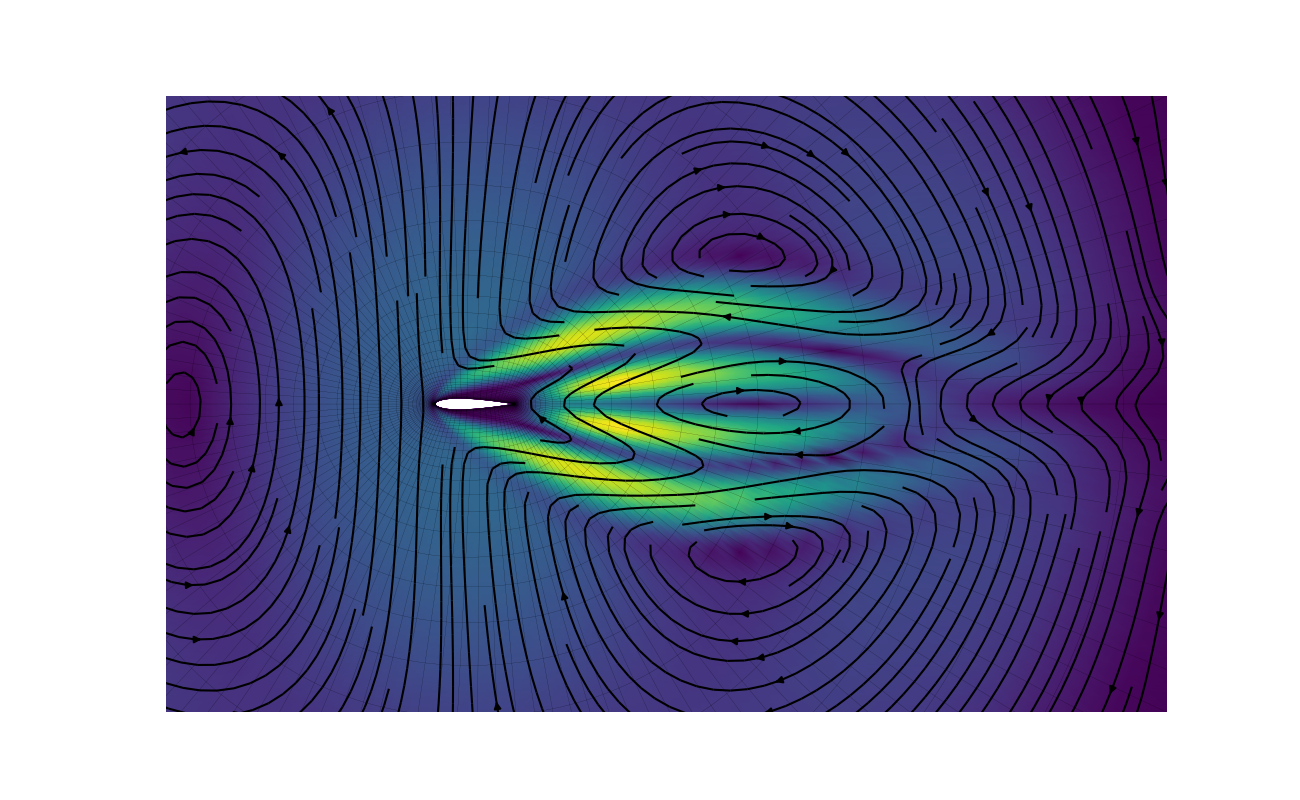
\includegraphics[width=1.0\textwidth]{figs/bfun-v-piola-v003}}
  \end{center}
\end{frame}

\begin{frame}
  \frametitle{Convergence}

  \begin{center}
    \begin{tikzpicture}
      \begin{axis}[
        xlabel={Expected mean relative error},
        ylabel={Mean relative error},
        ymode=log,
        xmode=log,
        width=0.9\textwidth,
        height=0.5\textwidth,
        grid=both,
        axis lines=left,
        legend style={
          at={(0.5, -0.3)},
          anchor=north,
          draw=none,
        },
        legend cell align=left,
        legend columns=4,
        ]
        \addplot[blue, thick, mark=*, mark options={solid}]
        table[x index={1}, y index={4}]{data/airfoil-results-no-piola-sups-no-block.csv};
        \addplot[blue, thick, densely dashed, mark=o, mark options={solid}]
        table[x index={2}, y index={8}]{data/airfoil-results-no-piola-sups-no-block.csv};
        \addplot[red, thick, mark=*, mark options={solid}]
        table[x index={1}, y index={4}]{data/airfoil-results-piola-sups-no-block.csv};
        \addplot[red, thick, densely dashed, mark=o, mark options={solid}]
        table[x index={2}, y index={8}]{data/airfoil-results-piola-sups-no-block.csv};
        \legend{TH ($v$), TH ($p$), DC ($v$), DC ($p$)}
      \end{axis}
    \end{tikzpicture}
  \end{center}
\end{frame}

\begin{frame}
  \frametitle{Convergence}

  \begin{center}
    \begin{tikzpicture}
      \begin{axis}[
        xlabel={Degrees of freedom ($M$)},
        ylabel={Mean relative error},
        ymode=log,
        width=0.9\textwidth,
        height=0.5\textwidth,
        grid=both,
        axis lines=left,
        legend style={
          at={(0.5, -0.3)},
          anchor=north,
          draw=none,
        },
        legend cell align=left,
        legend columns=4,
        ]
        \addplot[blue, thick, mark=*, mark options={solid}]
        table[x index={0}, y index={4}]{data/airfoil-results-no-piola-sups-no-block.csv};
        \addplot[blue, thick, densely dashed, mark=o, mark options={solid}]
        table[x index={0}, y index={8}]{data/airfoil-results-no-piola-sups-no-block.csv};
        \addplot[red, thick, mark=*, mark options={solid}]
        table[x index={0}, y index={4}]{data/airfoil-results-piola-sups-no-block.csv};
        \addplot[red, thick, densely dashed, mark=o, mark options={solid}]
        table[x index={0}, y index={8}]{data/airfoil-results-piola-sups-no-block.csv};
        \legend{TH ($v$), TH ($p$), DC ($v$), DC ($p$)}
        \draw[rounded corners=1mm, thick] (axis cs:28.5,0.0085) rectangle (axis cs:31.5,0.03);
      \end{axis}
    \end{tikzpicture}
  \end{center}
\end{frame}

\begin{frame}
  \frametitle{Convergence}

  \begin{center}
    \begin{tikzpicture}
      \begin{axis}[
        xlabel={Time (seconds)},
        ylabel={Mean relative error},
        ymode=log,
        xmode=log,
        width=0.9\textwidth,
        height=0.5\textwidth,
        grid=both,
        axis lines=left,
        legend style={
          at={(0.5, -0.3)},
          anchor=north,
          draw=none,
        },
        legend cell align=left,
        legend columns=3,
        ]
        \addplot[blue, thick, mark=*, mark options={solid}]
        table[x index={15}, y index={4}]{data/airfoil-results-no-piola-sups-no-block.csv};
        \addplot[blue, thick, densely dashed, mark=o, mark options={solid}]
        table[x index={15}, y index={8}]{data/airfoil-results-no-piola-sups-no-block.csv};
        \addplot[red, thick, mark=*, mark options={solid}]
        table[x index={11}, y index={4}]{data/airfoil-results-piola-sups-block.csv};
        \addplot[red, thick, densely dashed, mark=o, mark options={solid}]
        table[x index={11}, y index={8}]{data/airfoil-results-piola-sups-block.csv};
        \addplot[cyan, thick, mark=*, mark options={solid}]
        table[x index={11}, y index={4}]{data/airfoil-results-combined.csv};
        \addplot[cyan, thick, densely dashed, mark=o, mark options={solid}]
        table[x index={11}, y index={8}]{data/airfoil-results-combined.csv};
        \draw[rounded corners=1mm, thick] (axis cs:0.0255,0.009) rectangle (axis cs:0.035,0.032);
        \draw[rounded corners=1mm, thick] (axis cs:0.255,0.009) rectangle (axis cs:0.35,0.020);
        \draw (axis cs:0.0299,0.009) -- (axis cs:0.0299,0.003) -- (axis cs:0.299,0.003) -- (axis cs:0.299,0.009);
        \node[anchor=south] at (axis cs:0.18,0.003) {\boldmath$\times 10$};
        \legend{TH ($v$), TH ($p$), DC ($v$), DC ($p$), DC-LP ($v$), DC-LP ($p$)}
      \end{axis}
    \end{tikzpicture}
  \end{center}
\end{frame}

% \begin{frame}
%   \frametitle{Solutions}

%   \begin{center}
%     \only<1>{\includegraphics[height=0.6\textheight]{figs/no-piola-full}
%     }\only<2>{\includegraphics[height=0.6\textheight]{figs/piola-full}
%     }\only<3>{\includegraphics[height=0.6\textheight]{figs/no-piola-red}
%     }\only<4>{\includegraphics[height=0.6\textheight]{figs/piola-red}}
%     \\
%     \only<1>{Full TH solution: $39$ seconds.
%     }\only<2>{Full DC solution: $113$ seconds.*
%     }\only<3>{Reduced TH solution ($30$ DoFs): $523$ milliseconds.
%     }\only<4>{Reduced DC solution ($30$ DoFs): $96$ milliseconds.}
%   \end{center}
% \end{frame}

\begin{frame}
  \frametitle{Speedup factors}

  \begin{center}
    \bgroup\def\arraystretch{1.2}
    \begin{tabular}{crr}
      $\sharp$ DoFs ($M$) & {\bf Taylor-Hood} & {\bf Conforming} \\
      \hline $10$ & $1483$ & $6890$ \\
      $20$ & $390$ & $2616$ \\
      $30$ & $111$ & $1441$ \\
      $40$ & $52$ & $843$ \\
      $50$ & $27$ & $502$ \\
      \hline
    \end{tabular}
    \egroup
  \end{center}

\end{frame}

\begin{frame}
  \frametitle{Summary}
  \begin{itemize}
  \item Reduced order models offer dramatic speed-ups for certain applications.
  \item They combine nicely with IGA and div-compatible spaces to form fully
    divergence-free function spaces without need for pressure fields.
  \item Divergence-free RBMs can be much faster than other RBMs, in spite of additional complexity
    in the offline stage (remember, all is fair there.)
  \end{itemize}
  ~\\ \begin{center} Thank you! \end{center}
\end{frame}

\begin{frame}
  \frametitle{References}

  \printbibliography
\end{frame}

\end{document}
